\documentclass[a4paper]{article}

\usepackage[english]{babel}
\usepackage[utf8]{inputenc}
\usepackage{amsmath}
\usepackage{graphicx}
\usepackage{minted}
\usepackage{algorithm}
\usepackage[noend]{algpseudocode}
\usepackage[colorinlistoftodos]{todonotes}
\usepackage{multirow}
\usepackage{parskip}

% empty set package
\usepackage{amssymb}

% Automata package
\usepackage{pgf,tikz}
\usetikzlibrary{shapes,arrows,automata}


\title{CSCE 828 - Homework 3}
\author{Tian Gao}
\begin{document}
\maketitle

% Question 1
1. \\
$\because j > 3i$\\
$\therefore a^ib^j = a^ib^{3i}b^{j-3i}$\\
So the CFG for the language is:\\
$$
\begin{array}{rcr}
S_0&\rightarrow&S_1S_2\\
S_1&\rightarrow&aS_1bbb|\varepsilon\\
S_2&\rightarrow&S_2b|b
\end{array}
$$
$S_0 = a^ib^j, 3i < j, i\geqslant0,j\geqslant0$\\
$S_1 = a^ib^{3i}, i\geqslant0$\\
$S_2 = b^i,i > 0$\\

% Question 2
2.\\
$\because i\leqslant j \leqslant 3i$\\
$\therefore$ in each step of $S_0 \rightarrow a^xS_0b^y$, y is at least x and at most 3x\\
So the CFG for the language is:\\
$$
\begin{array}{rcr}
S_0&\rightarrow&aS_0b|aS_0bb|aS_0bbb|\varepsilon\\
\end{array}
$$
$S_0 = a^ib^j, i\leqslant j \leqslant 3i, i\geqslant0,j\geqslant0$\\

% Question 3
3.\\
$\because i < j < 3i$\\
$\therefore$ the answer is similar to question 2 but the map cannot always follow the path $S_0 \rightarrow aS_0b$ or $aS_0bbb$\\
So the CFG for the language is:\\
$$
\begin{array}{lcl}
S_0&\rightarrow&aS_1b|aS_2bb|aS_3bbb\\
S_1&\rightarrow&aS_2bb|aS_2bbb\\
S_2&\rightarrow&aS_2b|aS_2bb|aS_2bbb|\varepsilon\\
S_3&\rightarrow&aS_2b|aS_2bb\\
\end{array}
$$
$S_0 = a^ib^j, i < j < 3i, i\geqslant0,j\geqslant0$\\
$S_1 = a^ib^j, i < j \leqslant 3i, i\geqslant0,j\geqslant0$\\
$S_2 = a^ib^j, i\leqslant j \leqslant 3i, i\geqslant0,j\geqslant0$\\
$S_3 = a^ib^j, i\leqslant j < 3i, i\geqslant0,j\geqslant0$\\

% Question 4
4.\\
There are 3 cases:\\
case 1:$3i < j$, the answer is same as question 1\\
case 2:$i < j < 3i$, the answer is same as question 3\\
case 3:$j < i$, the answer is easy to get\\
So the CFG for the language is:\\
$$
\begin{array}{lcl}
S_0&\rightarrow&S_1|S_2|S_3\\

S_1&\rightarrow&S_4S_5\\
S_4&\rightarrow&aS_4bbb|\varepsilon\\
S_5&\rightarrow&S_5b|b\\

S_2&\rightarrow&aS_6b|aS_7bb|aS_8bbb\\
S_6&\rightarrow&aS_7bb|aS_7bbb\\
S_7&\rightarrow&aS_7b|aS_7bb|aS_7bbb|\varepsilon\\
S_8&\rightarrow&aS_7b|aS_7bb\\

S_3&\rightarrow&S_9|S_{10}\\
S_9&\rightarrow&aS_9b|\varepsilon\\
S_{10}&\rightarrow&aS_{10}|\varepsilon\\
\end{array}
$$
$S_0 = a^ib^j, i \neq j, 3i \neq j, i\geqslant0,j\geqslant0$\\
$S_1 = a^ib^j, 3i < j, i\geqslant0,j\geqslant0$\\
$S_2 = a^ib^j, i < j < 3i, i\geqslant0,j\geqslant0$\\
$S_3 = a^ib^j, j < i, i\geqslant0,j\geqslant0$\\
$S_4 = a^ib^{3i}, i\geqslant0$\\
$S_5 = b^i,i > 0$\\
$S_6 = a^ib^j, i < j \leqslant 3i, i\geqslant0,j\geqslant0$\\
$S_7 = a^ib^j, i\leqslant j \leqslant 3i, i\geqslant0,j\geqslant0$\\
$S_8 = a^ib^j, i\leqslant j < 3i, i\geqslant0,j\geqslant0$\\
$S_9 = a^ib^i,i > 0$\\
$S_{10} = a^i,i > 0$\\

% Question 5
5.\\
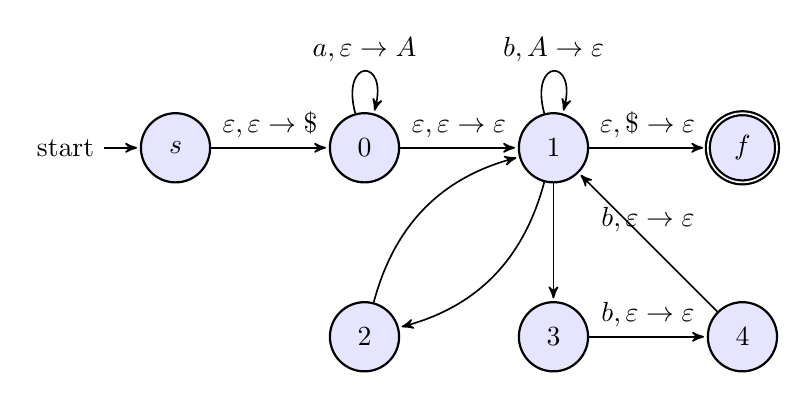
\begin{tikzpicture}[->,>=stealth',shorten >=1pt,auto,node distance=2.4cm,on grid,semithick, every state/.style={fill=blue!10,thick}]
\node[initial,state] 	 (s)              {$s$};
\node[state]        	 (0) [right of=s] {$0$};
\node[state]        	 (1) [right of=0] {$1$};
\node[state,accepting]   (f) [right of=1] {$f$};
\node[state]     		 (2) [below of=0] {$2$};
\node[state]  			 (3) [below of=1] {$3$};
\node[state]  			 (4) [below of=f] {$4$};
\path[->] 
	(s) edge [above]        node {$ \varepsilon , \varepsilon \rightarrow \$ $} (0)
	(0) edge [above]        node {$ \varepsilon , \varepsilon \rightarrow \varepsilon$} (1)
    (0) edge [loop above]   node {$ a,\varepsilon \rightarrow A $} (0)
	(1) edge [above]        node {$ \varepsilon, \$ \rightarrow \varepsilon $} (f)
    (1) edge [bend left]   		node {$  $} (2)
	(2) edge [bend left] 		node {$  $} (1)
	(1) edge [left] 	node {$  $} (3)  
    (1) edge [loop above]   node {$ b, A \rightarrow \varepsilon $} (1)
    (3) edge [above]   node {$ b, \varepsilon \rightarrow \varepsilon $} (4)
	(4) edge [above]		node {$ b, \varepsilon \rightarrow \varepsilon  $} (1);    
\end{tikzpicture}\\
How this PDA works:\\
For any given $s = a^ib^j, i\leqslant j \leqslant 3i, i\geqslant0,j\geqslant0$, \\ 
$\because i\leqslant j \leqslant 3i$\\
$\therefore$ j can be decomposed as $j = k_1+k_2+k_3+...+k_i, k_1,k_2,k_3,...,k_i \in \{1,2,3\}$\\
for $k_l, l=1,2,3,...,i$\\
if $k_l=1$, go along the path \textcircled{1} $\rightarrow$ \textcircled{1}\\
if $k_l=2$, go along the path \textcircled{1} $\rightarrow$ \textcircled{2} $\rightarrow$ \textcircled{1}\\
if $k_l=3$, go along the path \textcircled{1} $\rightarrow$ \textcircled{3} $\rightarrow$ \textcircled{4} $\rightarrow$ \textcircled{1}\\
$\therefore$ we can finally reach final state \textcircled{f}\\
$\therefore$ s can be accepted.\\

% Question 6
6.\\
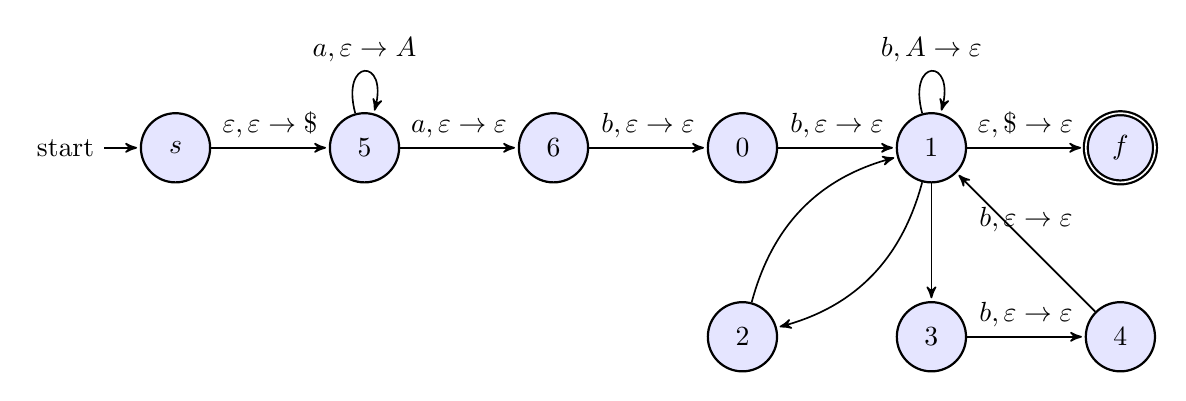
\begin{tikzpicture}[->,>=stealth',shorten >=1pt,auto,node distance=2.4cm,on grid,semithick, every state/.style={fill=blue!10,thick}]

\node[initial,state] 	 (s)              {$s$};
\node[state]        	 (5) [right of=s] {$5$};
\node[state]        	 (6) [right of=5] {$6$};
\node[state]        	 (0) [right of=6] {$0$};
\node[state]        	 (1) [right of=0] {$1$};
\node[state,accepting]   (f) [right of=1] {$f$};
\node[state]     		 (2) [below of=0] {$2$};
\node[state]  			 (3) [below of=1] {$3$};
\node[state]  			 (4) [below of=f] {$4$};
\path[->] 
	(s) edge [above]        node {$ \varepsilon , \varepsilon \rightarrow \$ $} (5)
	(5) edge [above]        node {$ a , \varepsilon \rightarrow \varepsilon $} (6)
	(6) edge [above]        node {$ b , \varepsilon \rightarrow \varepsilon $} (0)    
	(0) edge [above]        node {$ b , \varepsilon \rightarrow \varepsilon$} (1)
    (5) edge [loop above]   node {$ a,\varepsilon \rightarrow A $} (5)
	(1) edge [above]        node {$ \varepsilon, \$ \rightarrow \varepsilon $} (f)
    (1) edge [bend left]   		node {$  $} (2)
	(2) edge [bend left] 		node {$  $} (1)
	(1) edge [left] 	node {$  $} (3)  
    (1) edge [loop above]   node {$ b, A \rightarrow \varepsilon $} (1)
    (3) edge [above]   node {$ b, \varepsilon \rightarrow \varepsilon $} (4)
	(4) edge [above]		node {$ b, \varepsilon \rightarrow \varepsilon  $} (1);    
\end{tikzpicture}\\
How this PDA works:\\
For any given $s = a^ib^j, i < j < 3i, i\geqslant0,j\geqslant0$, \\ 
Consider :\\
case 1 : $j=2i$\\
case 2 : $i<j<2i$\\
case 3 : $2i<j<3i$\\
In each case, path $S \rightarrow aSbb$ must be included.\\
On the other hand, once path $S \rightarrow aSbb$ is included, we can turn $\{a^ib^j, i\leqslant j \leqslant 3i\}$ into $\{a^ib^j, i < j < 3i\}$\\
So we combine abb and $s = a^ib^j, i\leqslant j \leqslant 3i$\\
After reading a certain number of 'a'(\textcircled{5} $\rightarrow$ \textcircled{5})\\
There must be a 'abb'(\textcircled{6} $\rightarrow$ \textcircled{0} $\rightarrow$ \textcircled{1})\\
After that, similar to question 5, we can go along the path \textcircled{1} $\rightarrow$ \textcircled{1} or  \textcircled{1} $\rightarrow$ \textcircled{2} $\rightarrow$ \textcircled{1} or \textcircled{1} $\rightarrow$ \textcircled{3} $\rightarrow$ \textcircled{4} $\rightarrow$ \textcircled{1}\\
We can finally reach final state \textcircled{f}\\
$\therefore$ s can be accepted.\\

% Question 7
7.\\
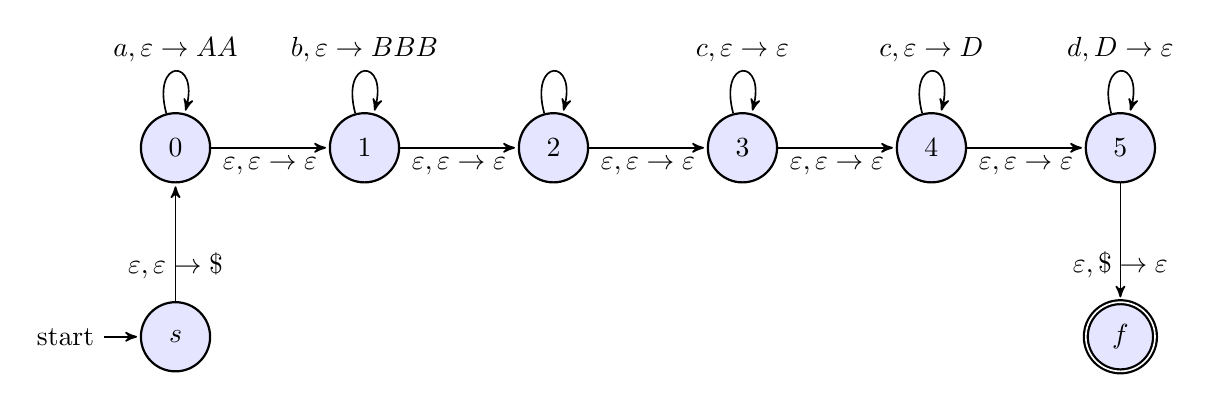
\begin{tikzpicture}[->,>=stealth',shorten >=1pt,auto,node distance=2.4cm,on grid,semithick, every state/.style={fill=blue!10,thick}]
\node[initial,state] 	 (s)              {$s$};
\node[state]        	 (0) [above of=s] {$0$};
\node[state]        	 (1) [right of=0] {$1$};
\node[state]     		 (2) [right of=1] {$2$};
\node[state]     		 (3) [right of=2] {$3$};
\node[state]     		 (4) [right of=3] {$4$};
\node[state]     		 (5) [right of=4] {$5$};
\node[state,accepting]   (f) [below of=5] {$f$};

\path[->] 
	(s) edge [below]        node {$ \varepsilon , \varepsilon \rightarrow \$ $} (0)
	(0) edge [below]        node {$ \varepsilon , \varepsilon \rightarrow \varepsilon$} (1)
    (1) edge [below]        node {$ \varepsilon , \varepsilon \rightarrow \varepsilon$} (2)
    (2) edge [below]        node {$ \varepsilon , \varepsilon \rightarrow \varepsilon$} (3)
    (3) edge [below]        node {$ \varepsilon , \varepsilon \rightarrow \varepsilon$} (4)
    (4) edge [below]        node {$ \varepsilon , \varepsilon \rightarrow \varepsilon$} (5)
    (5) edge [below]        node {$ \varepsilon, \$ \rightarrow \varepsilon $} (f)
    (0) edge [loop above]   node {$ a,\varepsilon \rightarrow AA $} (0)
    (1) edge [loop above]   node {$ b,\varepsilon \rightarrow BBB $} (1)
    (2) edge [loop above]   node {} (2)
    (3) edge [loop above]   node {$ c,\varepsilon \rightarrow \varepsilon$} (3)
    (4) edge [loop above]   node {$ c,\varepsilon \rightarrow D $} (4)
    (5) edge [loop above]   node {$ d,D \rightarrow \varepsilon$} (5)
	
;    
\end{tikzpicture}\\
How this PDA works:\\
$\because (2i+l)\leqslant(k-3j)$\\
$\therefore k \geqslant(2i+l+3j)$\\
$\therefore$ For any given $s = a^ib^jc^kd^l, (2i+l)\leqslant(k-3j), i,j,k,l\geqslant0$\\ 
$s = a^ib^jc^{2i+3j}c^{k-2i-3j-l}c^ld^l$\\
$\therefore$ after reading $a^i$, we can go along the path \textcircled{0} $\rightarrow$ \textcircled{0}\\
after reading $b^j$, we can go along the path \textcircled{1} $\rightarrow$ \textcircled{1}\\
after reading $c^{2i+3j}$, we can go along the path \textcircled{2} $\rightarrow$ \textcircled{2}\\
after reading $c^{k-2i-3j-l}$, we can go along the path \textcircled{3} $\rightarrow$ \textcircled{3}\\
after reading $c^l$, we can go along the path \textcircled{4} $\rightarrow$ \textcircled{4}\\
after reading $d^l$, we can go along the path \textcircled{5} $\rightarrow$ \textcircled{5}\\
$\therefore$ we can finally reach final state \textcircled{f}\\
$\therefore$ s can be accepted.\\

% Question 8
8.\\
The PDA is already in the special form.\\
The equivalent CFG has 3 $\times$ 3 variables. \\
The set of all variables V = $A_{p,q}$ where $1 \leqslant p \leqslant 3$ and $1 \leqslant q \leqslant 3$\\
The alphabet $\Sigma = \{a,b\}$\\
The start variable $S = A_{1,3}$\\
The set of all rules R is followed.\\
$$01.A_{1,1} \rightarrow A_{1,1}A_{1,1}$$
$$02.A_{1,1} \rightarrow A_{1,2}A_{2,1}$$
$$03.A_{1,1} \rightarrow A_{1,3}A_{3,1}$$
$$04.A_{1,2} \rightarrow A_{1,1}A_{1,2}$$
$$05.A_{1,2} \rightarrow A_{1,2}A_{2,2}$$
$$06.A_{1,2} \rightarrow A_{1,3}A_{3,2}$$
$$07.A_{1,3} \rightarrow A_{1,1}A_{1,3}$$
$$08.A_{1,3} \rightarrow A_{1,2}A_{2,3}$$
$$09.A_{1,3} \rightarrow A_{1,3}A_{3,3}$$
$$10.A_{2,1} \rightarrow A_{2,1}A_{1,1}$$
$$11.A_{2,1} \rightarrow A_{2,2}A_{2,1}$$
$$12.A_{2,1} \rightarrow A_{2,3}A_{3,1}$$
$$13.A_{2,2} \rightarrow A_{2,1}A_{1,2}$$
$$14.A_{2,2} \rightarrow A_{2,2}A_{2,2}$$
$$15.A_{2,2} \rightarrow A_{2,3}A_{3,2}$$
$$16.A_{2,3} \rightarrow A_{2,1}A_{1,3}$$
$$17.A_{2,3} \rightarrow A_{2,2}A_{2,3}$$
$$18.A_{2,3} \rightarrow A_{2,3}A_{3,3}$$
$$19.A_{3,1} \rightarrow A_{3,1}A_{1,1}$$
$$20.A_{3,1} \rightarrow A_{3,2}A_{2,1}$$
$$21.A_{3,1} \rightarrow A_{3,3}A_{3,1}$$
$$22.A_{3,2} \rightarrow A_{3,1}A_{1,2}$$
$$23.A_{3,2} \rightarrow A_{3,2}A_{2,2}$$
$$24.A_{3,2} \rightarrow A_{3,3}A_{3,2}$$
$$25.A_{3,3} \rightarrow A_{3,1}A_{1,3}$$
$$26.A_{3,3} \rightarrow A_{3,2}A_{2,3}$$
$$27.A_{3,3} \rightarrow A_{3,3}A_{3,3}$$
$$28.A_{1,3} \rightarrow A_{2,2}$$
$$29.A_{2,2} \rightarrow aA_{2,2}b$$
$$30.A_{2,2} \rightarrow bA_{2,2}a$$
$$31.A_{1,1} \rightarrow \varepsilon$$
$$32.A_{2,2} \rightarrow \varepsilon$$
$$33.A_{3,3} \rightarrow \varepsilon$$

% Question 9
9.\\
Assume that L is context free and let p be the pumping length.\\
Let $s =  " 0^p1^p1^p0^P " \in L$ .\\
$\therefore |s| \geqslant p$ \\
$\therefore s=uvxyz$ where $|uv|>0$ and $|vxy| <= p$ (According to Pumping Lemma)\\
There are 3 cases:\\
1. vy is in the form of $0^i1^j$. \\
$\therefore s'=uv^0xy^0z$ is not palindromes. \\
$\therefore s'\notin L$\\
2. vy is in the form of $1^i0^j$. \\
$\therefore s'=uv^0xy^0z$ is not palindromes. \\
$\therefore s'\notin L$\\
3. vy is in the form of $1^i$. \\
$\therefore s'=uv^0xy^0z$ has less 1s than 0s. \\
$\therefore s'\notin L$\\
However, according to Pumping Lemma, $s'\in L$\\
So the assumption is wrong and L is not context free.\\

% Question 10
10.\\
Assume that L is context free and let p be the pumping length.\\
Let $s =  " a^pb^p\#a^pb^P\# " \in L$ .\\
$\therefore |s| \geqslant p$ \\
$\therefore s=uvxyz$ where $|uv|>0$ and $|vxy| <= p$ (According to Pumping Lemma)\\
There are 2 cases:\\
1. vy contains $\#$ \\
$\therefore s'=uv^0xy^0z$ has less than 2\#. \\
$\therefore s'\notin L$\\
2. vy doesn't contain \#, there are also 3 sub cases\\
2.1 vy locates before the 1st \#\\
$s'=uv^0xy^0z$ has no $x_j=x_k$\\
$\therefore s'\notin L$\\
2.2 vy locates between the 1st \# and the 2nd \#\\
$s'=uv^0xy^0z$ has no $x_j=x_k$\\
$\therefore s'\notin L$\\
2.3 v locates before the 1st and y locates between the 1st \# and the 2nd \#\\
$\therefore v contains only b and y contains only a$\\
$s'=uv^0xy^0z$ has no $x_j=x_k$\\
$\therefore s'\notin L$\\
However, according to Pumping Lemma, $s'\in L$\\
So the assumption is wrong and L is not context free.\\













\end{document}